\section{Model Fragmentation}
\label{sec:fragmentation}

\subsection{Fragmention in General}
As briefly mentioned before, all models considered in this paper can be characterizes as directed labled graphs with a fix spanning-tree (\emph{containment hierarchy}). In EMF based models, these trees consist of \emph{containment references}. The meta-model determines, which references are containment references and which are simply \emph{cross-references} through the use of \emph{containment reference} or \emph{cross-reference features}.

In the last section, we saw that typical model applications mostly use aggregates of model objects, more precisely sub-trees of the model's containment hierarchy. We propose model fragmentation. The model fragmentation approach, divides (i.e. \emph{fragments}) a model along its containment hierarchy. All \emph{fragments} are disjoint; no object is part of two fragments. Fragmentation is also always complete, i.e. each object is part of one fragment. The set of fragments of a model is called \emph{fragmentation}. Based on these characteristics, fragments can be compared to EMF's resources (especially with containment proxies); refer to section~\ref{sec:implemention}, where we use resources to realize fragmentation. Fig.~\ref{fig:metamodel_fragmentation_pattern_tree} and Fig.~\ref{fig:metamodel_fragmentation_pattern_graph} present two examples.


\begin{figure}[ht]
\begin{minipage}[b]{0.5\linewidth}
\centering
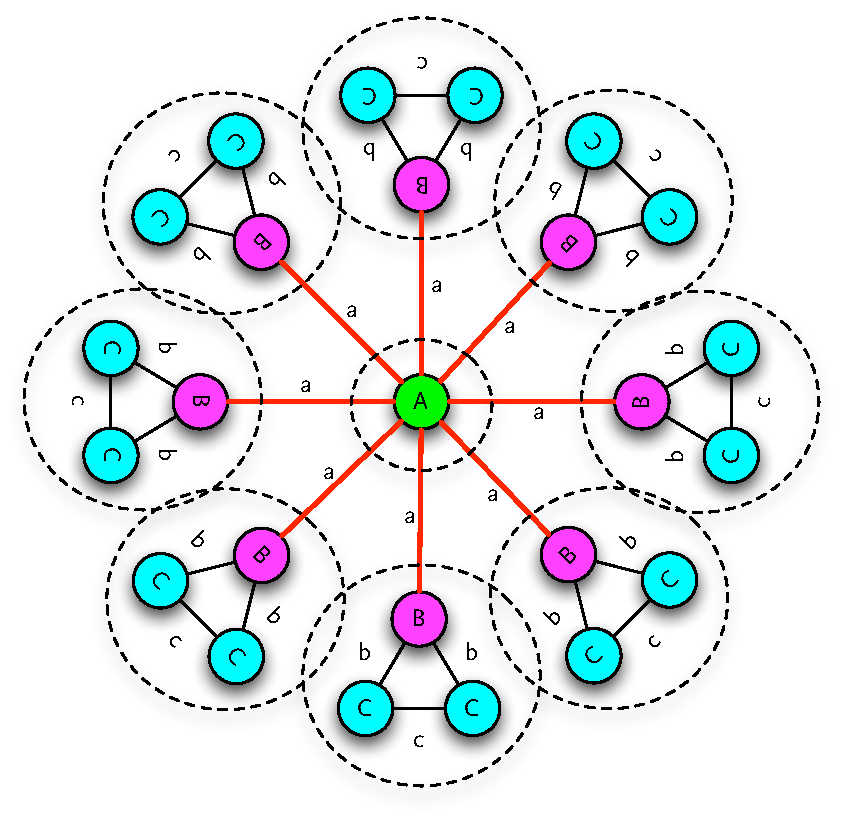
\includegraphics[width=\linewidth]{figures/metamodel_fragmentation_patterns_tree}
\caption{A fragmented example  model with classes A,B,C and reference features a,b,c. Fragments are denotes with circles, references with lines: black for intra- and red for inter-fragment references.}
\label{fig:metamodel_fragmentation_pattern_tree}
\end{minipage}
\hspace{0.5cm}
\begin{minipage}[b]{0.5\linewidth}
\centering
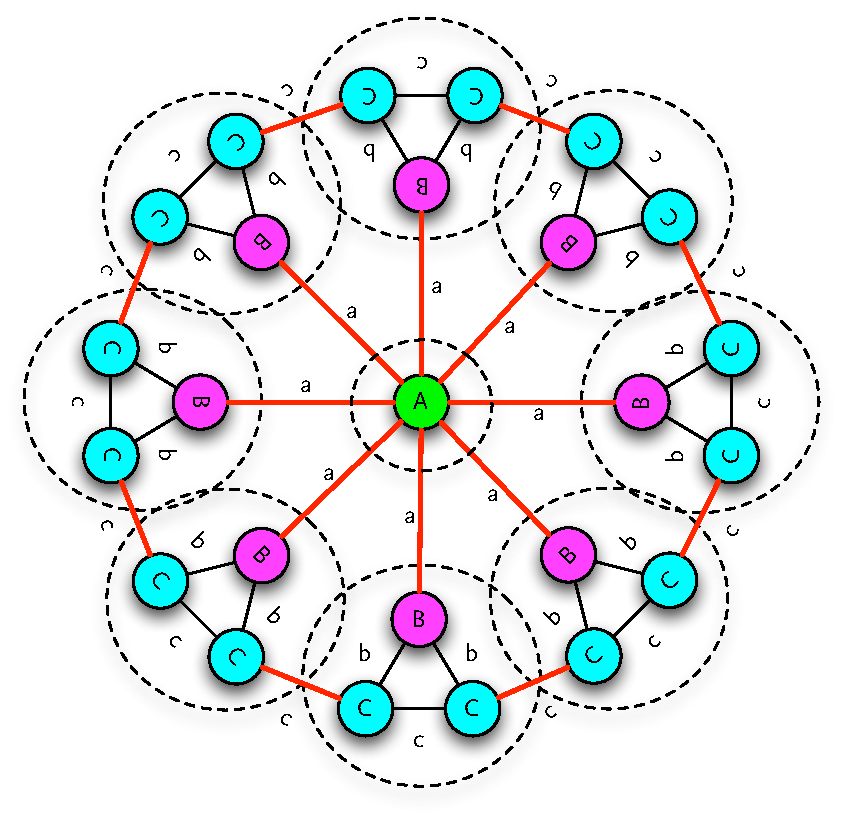
\includegraphics[width=\linewidth]{figures/metamodel_fragmentation_patterns_graph}
\caption{This example contains inter-fragment cross-references (feature c), i.e. inter-fragment references \emph{by accident}. Feature a produces inter-fragment containment references.}
\label{fig:metamodel_fragmentation_pattern_graph}
\end{minipage}
\end{figure}  

\subsection{Fragmentation Strategies}

Originally a model has no fragmentation; also do we need to maintain a fragmentation when a model is manipulated. Further, we have to assume that fragmentation has an influence on performance. We denote algorithms necessary to create and maintain a fragmentation as \emph{fragmentation strategies}.

There are two trivial strategies: \emph{no fragmentation} and \emph{total fragmentation}. No fragmentation means the whole model constitutes the one and only fragment, such as in regular EMF (without resources). Total fragmentation means each object constitutes its own fragment. There are as many fragments as objects in the model. This strategy is implemented by existing persistence frameworks.

\subsection{Meta-Model based Fragmentation}

There are other fragmentation strategies that produce fragmentations between no and total fragmentation. In this paper, we propose and use \emph{meta-model based fragmentation} as a new (but very simple) strategy.

A meta-model defines possible models by means of classes and associations (i.e. structural features in EMF). A good meta-model only allows models that are suitable for the envisioned application. Containment references (indirectly the containment hierarchy) are already used by the meta-modeller to aggregate\footnote{In UML composition is a special case of aggregation} closely related objects. For the meta-model based fragmentation strategy, we ask the meta-modeller to mark some containment reference features as \emph{inter-fragment reference features}. All instances of these features, will break the containment hierarchy into fragments (we call their instances \emph{inter-fragment} references). This way, the meta-model determines where the spanning-tree is broken into fragments. 
Once inter-fragment reference features are designated within the meta-model, it is easy to create and maintain fragmentations automatically and transparently; ref. to section~\ref{sec:implemention}.

Only containment features can be designated as inter-fragment reference features and all instances of such a reference feature will be inter-fragment references (like \texttt{a}-references in Fig.~\ref{fig:metamodel_fragmentation_pattern_tree}). Other references (i.e. cross references) can become inter-fragment references \emph{by accident} (like \texttt{c}-references in Fig.~\ref{fig:metamodel_fragmentation_pattern_graph}).


%\subsubsection{Theory}
%Access patterns for a model are strongly influenced by its metamodel.
%Metamodels are tiny in comparison to their large instances. 
%If you imagine looking from above onto a large model, the metamodel types of its objects form patterns. How we access a model is also influenced by its metamodel, since all algorithms doing something with a model are programmed against its metamodel.
%Hence, optimal fragmentation goes along this patterns.
%Most fragments will have the same structure, and fragments are connected through structural features of only few different types.
%One way to define fragmentation is to mark these fragment crossing structural features. 
%
%Fig.~\ref{fig:metamodel_fragmentation_pattern_tree} shows a simple example metamodel type pattern. The instances (links) of feature \emph{a} cross fragment borders (inter fragment links). All other links are intra-fragment links. The situation is a  little more complicated in Fig.~\ref{fig:metamodel_fragmentation_pattern_graph}. Here the links of feature \emph{c} have both inter- and intra-fragment instances. 
%
%If we want to describe fragmentation by marking features as inter- or intra-fragment features, it would work for the example in Fig.~\ref{fig:metamodel_fragmentation_pattern_tree}, but not for the example in Fig.~\ref{fig:metamodel_fragmentation_pattern_graph}. Obviously, we need further restrictions.
%
%Models (as used in this paper) always have a inherent spanning tree. The spanning tree is formed from links that are instances from containment features. All instances of containment features are part of the spanning tree. If we only allow containment features to be inter-fragment features then the instances of inter-fragment feature will always define a unique fragmentation. \markus{Proof?}
%
%\subsubsection{Implementation}
%This describes an implementation based on EMF. 
%
%\subsection{Automated Fragmentation based on Expected Range Queries}
%\subsection{Automated Fragmentation based on Access Patterns}
%\subsection{Fragmentation of Even Models}
%
%\subsubsection{Analysis}
%
%At the beginning, we will look at \emph{even} models. A model is even, if its inner structure suggest fragmentation into equal pieces. For example, an intuitive way to fragment a OO software model is to put each package into one entry. This is an uneven model, since packages have different sizes. Another example is sensor data, sensor data produced at each point in time or on each node has the same size. If one puts each sensor reading or each node into one entry, the entries will have similar size.
%
%Previously, we were looking the gains achieved with optimal fragmentation. While optimal fragmentation is plausible in manually fragmented models for a single specific loaded model (e.g. accessing single sensor readings in ClickWatch). Optimal fragmentation is unlikely for different loaded models (even impossible for models of different size). 
%
%In general, we can assume that the smaller $ope$ is compared to $load$, the more likely it is that much of each entry is part of the loaded model. In other words, the smaller my entries are, the more likely it is that much or all if a single entry is part of the loaded model. We will model $part$  accordingly.